\chapter{Jet Energy Scale}
\label{JES}

Recalling from Sec.~\ref{jets} that jets evolve through many different stages (see Fig.~\ref{JetLevelsFig}) it becomes clear that to reasonably compare experimental results to theoretical results one must decide on a scale at which to make the comparison.  
This also allows for comparisons that do not require any knowledge of the detector itself.  
This is usually done by bringing all results to the ``particle jet'' or ``truth jet'' scale, as described in Sec.~\ref{Sec:JetFinding}.  
This makes the results detector independent easing cross experiment comparisons.  
This is accomplished by carefully studying the relationship between the particle scale jet energy and the detector scale jet energy, known as the \gls{JES}.   
A successful \gls{JES} accounts for pileup, escaped/invisible energy, algorithm effects, etc.  


\begin{figure}[!ht]
  \begin{center}
    \scalebox{0.40}{
      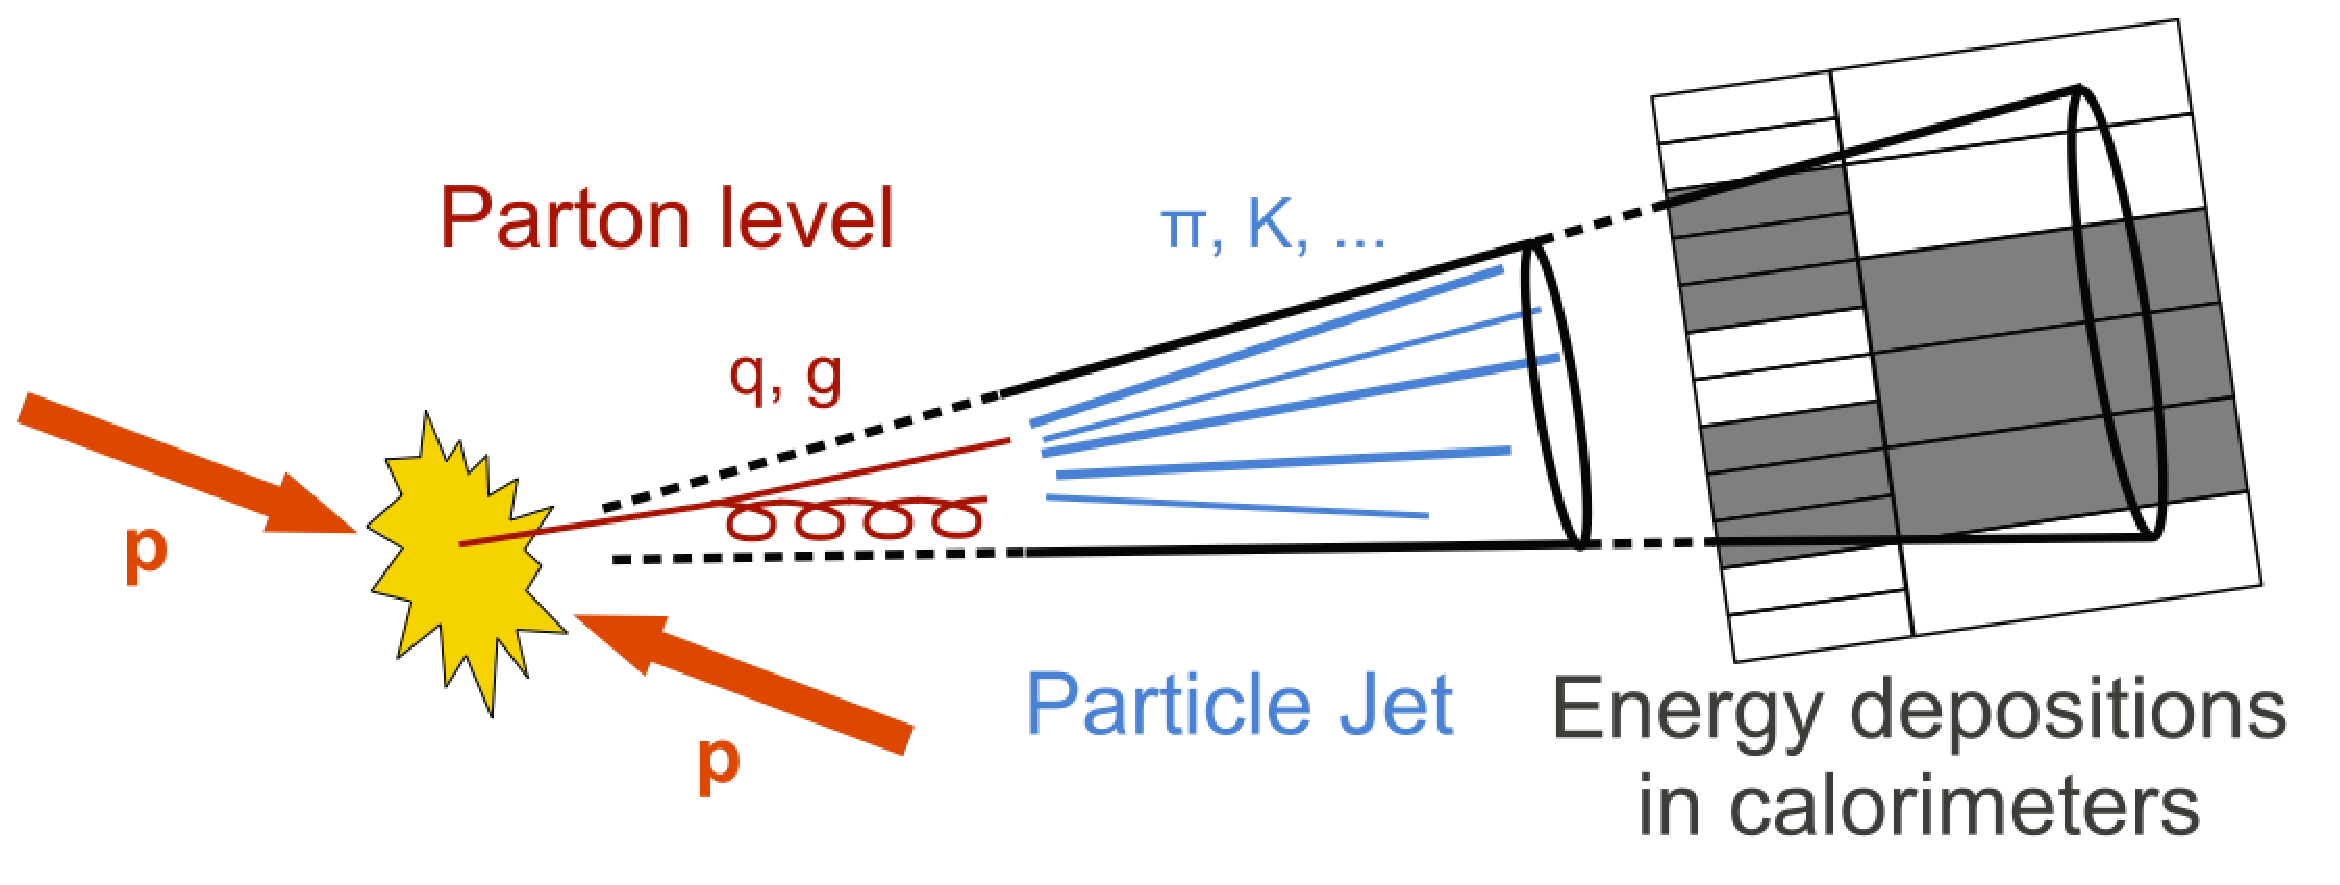
\includegraphics{plots/Chap4/Sketch_PartonParticleCaloJet.eps}
    }
  \end{center}
  \caption[Jet showering evolution.]
      {\small A diagram outlining the progression from parton level to a calorimeter jet.}
  \label{JetLevelsFig}
\end{figure}

\section{Jet Energy Scale in ATLAS}
\label{ATLASJES}

Calibrating jets at ATLAS is a multistaged process.  
During the initial jet reconstruction the jet is set to originate from point (0,0,0) in the ATLAS coordinate system, so the first step is to adjust the jet to originate from the reconstructed vertex using the tracking information.  
Next in order to compensate for energy coming adjacent beam bunches and secondary interactions in the same beam bunch crossing (pileup) energy is subtracted from the jet, first using the average energy density observed in that given event multiplied by the active area of the jet.  
The area of a jet is determined by adding a large number of equally spaced particles with infinitesimally small energy (called ghost particles, see~\cite{Soyez:2012hv}) to the event and rerunning the jet reconstruction algorithm.  
The number of ghost particles in a given jet is used to determine its area.  
This subtraction is followed by two residual corrections, which are applied to completely remove the jet energy's dependence on pileup.  
One correction is based on the average number of interactions in neighbouring beam bunches and another is based on the actual reconstructed number of interactions in that given event.    
With pileup now removed a Monte Carlo based calibration, which completely corrects for the average response as a function of energy and pseudorapidity of the jet, is applied.  

To improve the energy resolution and reduce the flavour dependence of the jets at this stage a series of smaller Monte Carlo based calibration factors are applied.  
These ideally flatten the dependence of the response on the amount of energy in the first layer of the hadronic calorimeter, the energy in the last layer of the EM calorimeter, the number of charged tracks in the jet, the width of the distribution of the tracks in the jet, and the number of track segments in the muon spectrometer behind the jet.  
These calibrations are collectively known as the \gls{GSC} scheme.  

\begin{figure}[!ht]
  \begin{center}
    \scalebox{0.40}{
      \includegraphics{plots/Chap4/CalibSequence.ps}
    }
  \end{center}
  \caption[Jet calibration sequence used by ATLAS.]
      {\small A diagram outlining the progression from a calorimeter jet back to a particle level jet.  }
  \label{Fig:JetCalibSequenceFig}
\end{figure}


The last step involves applying final corrections to account for the observed differences in response between the data which have been collected and the Monte Carlo simulations.  
The response is measured using a series of \textit{in-situ} techniques in both data and Monte Carlo, and the ratio is applied as a final factor to complete the calibration of the data.  
In general these \textit{in-situ} techniques make use of transverse momentum balance in a system of physics objects that have been produced back-to-back in $\phi$.  
One object, which is well measured, is labeled as the reference object and the response of the second object is measured relative to it.  
These studies can be performed in dijet events where the jets land in different $\eta$ regions, which is done to transfer the jet calibration from one part of the detector to another (so called eta intercalibration), $\gamma$/Z+jet events where the jet response is measured relative to the boson to give the absolute JES, and multi jet events where one high energy jet is measured relative to several previously calibrated lower energy jets to extend the calibration to energies where the $\gamma$/Z+jet cross-section is too small to be useful.  

This thesis presents work using both Z+jet and $\gamma$+jet events to study the jet energy scale in ATLAS.  
Only events where the Z decays into either an electron/positron pair or a muon/anti-muon pair are considered.  
When it comes to measuring the JES these two types of events are similar and complementary.  
Both offer well-measured objects that are ideally produced back-to-back in $\phi$ with a single jet, with a significant difference being that the cross section for $\gamma$+jet is several orders of magnitude larger.   
This larger cross section allows for a larger number of high energy $\gamma$+jet events, increasing the range that can be calibrated.  
Unfortunately this larger cross section also forces lower energy photon triggers to be prescaled to much lower rates.  
This prescaling at low energy combined with the large number of low energy dijet events being misidentified as $\gamma$+jet events makes Z+jet a much better choice to calibrate the low energy regime.  

\section{Jet Response}
\label{sec:JetResponse}
The largest component of the JES correction is the absolute response, which describes how the calorimeter responds to both hadronic and electromagnetic energy deposits within the jet.  
Even for a single incoming hadron there will be some fraction of energy deposited in the calorimeter via EM interactions.  
This is in part because hadrons have electric charge, but is largely due to hadrons producing particles in the calorimeter that decay electromagnetically ($\pi^0\rightarrow\gamma\gamma$).  
The single-particle response (defined as $E^{\mathrm {measured}} / E^{\mathrm {truth}}$) can be written in terms of these two types if energy deposits as follows:

\begin{equation}
  \label{SingleParticleResponse}
  r(E)=f_{\mathrm{em}}\left(E\right)e+\left[1-f_{\mathrm{em}}\right]\left(E\right)h,
 \end{equation}

\noindent
where $e$ is the response to purely EM energy deposits, $h$ is the response to purely hadronic energy deposits, and $f_{\mathrm{em}}$ is the fraction of the total incoming energy that is deposited electromagnetically.  

This can be further explored by using a simplistic model of a particle showering within a material.  
When a hadron interacts with a nucleus several new hadrons are created, with pions being produced in the largest numbers.  
Thanks to the (slightly broken) isospin symmetry of hadronic interactions each flavour of pion is created with equal probability, so if only pions are produced in a given interaction on average 1/3 of them will be electromagnetically decaying neutral pions.  
With this model in mind after the first generation of hadrons is produced 1/3 of the available energy is electromagnetic in nature, deposited by photons resulting from the decay of neutral pions.  
If the charged pions making up the remaining 2/3 of the original available energy each have enough energy to cause subsequent nuclear interactions, a further 2/9$^{\mathrm{ths}}$ of the energy is deposited electromagnetically, and so on.  
This dependence of the fraction of EM energy on the total energy of the incident particle can be modeled using

\begin{equation}
  \label{Grooms}
  f_{\mathrm{em}}\left(E\right)=1-\left(\frac{E}{E_0}\right)^{m-1}.
\end{equation} 

\noindent 
Another function that has been used to model the EM fraction with success is 
\begin{equation}
  \label{Wigmans}
  f_{\mathrm{em}}\left(E\right)=a_0+a_1\mathrm{ln}\frac{E}{E_{\mathrm{scale}}}, 
%+a_2\left(\mathrm{ln}\frac{E}{E_{\mathrm{scale}}}\right)^2, 
\end{equation}
\noindent
where variations including higher orders of $\mathrm{ln}\frac{E}{E_{\mathrm{scale}}}$ have been used as well, with ATLAS previously including both $\mathrm{ln}\left(\frac{E}{E_{\mathrm{scale}}}\right)^2$ and $\mathrm{ln}\left(\frac{E}{E_{\mathrm{scale}}}\right)^3$ terms into their fit~\cite{ATLAS-CONF-2010-056}~\cite{ATLAS-CONF-2011-032}.  
The response of an entire jet ($R_{\mathrm{jet}}$) can be expressed as 
\begin{equation}
  R_{\mathrm{jet}}\left(E\right)=w_h\,r\left(w_h\,E\right)+w_e\,e\left(w_e\,E\right)
\end{equation}
\noindent 
along with Eq.~\ref{SingleParticleResponse} and either Eq.~\ref{Grooms} or Eq.~\ref{Wigmans}, where $w_h$ and  $w_e$ are the fractions of particles in the jet incident on the calorimeter that interact hadronically or electromagnetically, respectively.  
These quantities are solely dependent on the parton shower and hadronization processes and are independent of any subsequent showering within the detector.   

\section{$E_{\mathrm T}^{miss}$ Projection Fraction Method}
\label{METProj}

The Missing $E_{\mathrm T}$ projecting fraction (MPF) method is an \textit{in-situ} technique for measuring the jet response.  
It was first developed at the CDF collaboration~\cite{abe1992dijet} to help with their $\eta$ intercalibration, and was also used by the D0 collaboration to extract an absolute jet energy scale~\cite{item/10150/186444}.  
In contrast to the $p_{\mathrm T}$ balance method, which directly compares the measured energy of the jet to the reference object, the MPF measures the response of the calorimeter to the entire recoiling system.

The MPF does this using only the measured reference (or probe) energy and the MET, removing the need to explicitly include the measured jet energy in the response measurement making it independent of the jet algorithm that was used.  
It should be noted that the response still depends on the inputs to the jet finding algorithm, and therefore a MET calculated at the appropriate scale must be used.  
This absence of jet information in the calibration means that to perform a full \textit{in-situ} calibration additional algorithm/jet size related corrections need to be derived.  
This deficiency is compensated by the fact that the MPF method is much more resilient to initial/final state radiation, which allows for looser event selection criteria resulting in a relatively larger sample size.  
Furthermore, the MPF technique is relatively unaffected by pileup.  

The MPF takes advantage of the balance between the reference object and the recoiling parton to obtain a measure of the true momentum in the recoil, so the derivation of the MPF response begins with 
\begin{equation}
  \label{EQ:MPFPartonLevel}
  \vec{p}_{\mathrm T}^{\mathrm{ref}}+\vec{p}_{\mathrm T}^{\mathrm{recoil}} = 0.  
\end{equation}
\noindent
where $\vec{p}_{\mathrm T}$ is the total momentum of a given particle/object projected into the transverse plane.   
This momentum balance must also be considered at the calorimeter level, which in the simple case of a $2\rightarrow$2 collision can be written as
\begin{equation}
  \label{EQ:MPFCaloLevel}
  R_{\mathrm{ref}}\vec{E}_{\mathrm T}^{\mathrm{ref}}+R_{\mathrm{recoil}}\vec{E}_{\mathrm T}^{\mathrm{recoil}}=-\vec{E}_{\mathrm T}^{\mathrm{miss}},
\end{equation}
\noindent
where we are using $R_{\mathrm{object}}$ to be the response of the calorimeter to that object and $\vec{E}_{\mathrm T}^{\mathrm{miss}}$ results from the fact that $R_{\mathrm{ref}} \neq R_{\mathrm{recoil}}$.  
We have also assumed that the masses of the particles in question are small compared to the energies involved to we approximate $\vec{p}=E\hat{p}$.  
$\vec{E}_{\mathrm T}^{\mathrm{object}}$ is known as the transverse energy of the object which is defined as
\begin{equation}
  \vec{E}_{\mathrm T}=\frac{E}{\mathrm{cosh}\left(\eta\right)}\hat{p}_{\mathrm T}.  
\end{equation}
\noindent
In this thesis only well measured objects are used as references, so $R_{\mathrm{ref}}\simeq1$ and small differences are well known and can be propagated to $\vec{E}_{\mathrm T}^{\mathrm{miss}}$.  
By projecting both sides of Eq.~\ref{EQ:MPFCaloLevel} along the direction of the reference object and using Eq.~\ref{EQ:MPFPartonLevel} to remove ${E}_{\mathrm T}^{\mathrm{recoil}}$ we obtain
\begin{equation}
  E_{\mathrm T}^{\mathrm{ref}}-R_{\mathrm{recoil}}E_{\mathrm T}^{\mathrm{ref}}=-\vec{E}_{\mathrm T}^{\mathrm{miss}}\cdot\hat{p}_{\mathrm T}^{\mathrm{ref}}.
\end{equation} 

\begin{equation}
  \label{EQ:MPFSimple}
  R_{\mathrm{recoil}}=1+\frac{\vec{E}_{\mathrm T}^{\mathrm{miss}}\cdot\hat{p}_{\mathrm T}^{\mathrm{ref}}}{E_{\mathrm T}^{\mathrm{ref}}}.
\end{equation}

This variable, referred to henceforth as MPF, is used to measure the JES \textit{in-situ}.  
What exactly the MPF measures can be made more clear by expanding out the MET.  
In the ideal case where only the reference object and the recoil exist (using Eq.~\ref{EQ:MPFCaloLevel}) we get that the MPF is just the ratio of the measured energy of the recoil to the measured energy of the reference object, so it measures the response of the calorimeter to the particles making up the recoil.  
In practice the MET includes particles radiated by the partons participating in the hard scattering (before and after the interaction), known as initial and final state radiation (ISR and FSR), as well as the underlying event (all particles in the initial protons which to not participate in the hard scattering), and pileup.  
This means that the MET can be written as 
\begin{equation}
  \vec{E}_{\mathrm T}^{\mathrm{miss}} = -\vec{E}_{T}^{\mathrm{ref}}-\sum_{n}\vec{E}_{\mathrm T}^{n},
\end{equation}
where n runs over all energy deposits in the calorimeter that are not related to the reference object.  
Using this definition of the MET we see that the MPF (as measured) can be written as 
\begin{equation}
  R_{\mathrm{recoil}}=1-\frac{E_{\mathrm T}^{\mathrm{ref}}+\hat{p}_{\mathrm T}^{\mathrm{ref}}\cdot\sum_{n}\vec{E}_{\mathrm T}^{n}}{E_{\mathrm T}^{\mathrm{ref}}}=-\frac{\sum_{n}\vec{E}_{\mathrm T}^{n}\cdot\hat{p}_{\mathrm T}^{\mathrm{ref}}}{E_{\mathrm T}^{\mathrm{ref}}}.
\end{equation}
In this form it is much clearer that the MPF is in fact balancing all energy in the event against the reference object.  
Although at first this may seem like a potentially large problem for the MPF to overcome thankfully this is not the case.  
Both the pileup, and to a lesser extent the underlying activity, are uncorrelated with the hard scattering.  
This means that while this extra energy may raise or lower the measured response on an event by event basis when measured over a large sample they will average out to zero (to first order).  
It will be shown in this thesis that the effects of these extra effects are small and can for the most part be ignored.  
As seen in Fig.~\ref{Fig:JetCalibSequenceFig} the ATLAS collaboration uses these \textit {in-situ} JES studies as a residual correction to a MC based calibration.  

\section{Jet Showering}
\label{sec:ShoweringIntro}
The idealized event topology used to derive the MPF equation ignored the potential effects of a number of subtle issues which have the potential to affect the accuracy of a calibration derived using this method.
One of these issues is the assumption that the response of the full hadronic recoil is the same as the response of jet which is reconstructed at the centre of the recoil.
While the majority of the energy of the recoil does reside within a narrow core (the jet) there are contributions from a diffuse halo of mostly low energy particles outside of the jet but still related to the recoil.  
This small amount of energy from lower energy particles has a lower response than the high energy particles in the core, an effect made more significant by the noise suppressing nature of the topo-clustering algorithm.
%This means that preforming a full {\textit {in-situ}} calibration using the MPF method would require the presence of an additional correction to compensate for this difference.  
%This correction is referred to as the jet topology correction, or simply the topology correction.  

Another issue is that the MPF is designed the measure the response of the full hadronic recoil in the calorimeter, that does not include a measure of the flow of energy in the calorimeter shower across the boundaries drawn by the jet reconstruction algorithm.
This means that not all of the energy within the reconstructed calorimeter jet necessarily originated from particles in the particle/truth jet, and likewise there is no guarantee that all of the energy deposited by particles in the truth jet is reconstructed within the calorimeter jet.
While a $p_{\mathrm T}$ balance based calibration inherently measures and compensates for any potential flow of energy across the boundaries of the jet, an MPF-based calibration (being jet algorithm independent) does not.

These two issues could be covered by a single correction, but that correction would provide no insight into the underlying physics.  
Instead they will be treated independently as the showering correction, which deals with the flow of energy across the jet boundary and is mostly effected by the low energy nuclear physics modeling, and the topology correction, which deals with the difference between the jet response and the recoil response and can be affect by both perturbative and non-perturbative QCD modelling.  
To define these corrections the so-called ``true calorimeter response'' is introduced.  
It is defined as 
\begin{equation}
  R_{\mathrm{true}} = \frac{\sum_{i\in{\mathrm{particle~jet}}} E_i^{\mathrm{measured}}}{\sum_{i\in{\mathrm{particle~jet}}}E_i^{\mathrm{true}}}, 
\end{equation}
\noindent
that is to say the sum of the energy measured in the calorimeter that originates from particles within the particle/truth jet divided by the total energy of the particle jet.  
Using this definition for the true calorimeter response the topology correction is defined as
\begin{equation}
  k_{\mathrm{topo}} = \frac{R_{\mathrm{MPF}}}{R_{\mathrm{true}}}
\end{equation}
\noindent
This isolates the question relating the full hadronic response to the response of the dense energy core.
In addition a ``showering'' correction can now be defined as 
\begin{equation}
  S = \frac{R_{\mathrm{true}}}{R_{\mathrm{jet}}}.  
\end{equation}
\noindent
This showering correction solely focuses on the flow of energy across the boundary of the calorimeter jet.


